\documentclass{article}
\usepackage{graphicx}
\usepackage{amsmath}
\usepackage{amssymb}
\usepackage{fullpage}
\title{6.867 Problem Set 1}
\date{October 1, 2015}

\begin{document}
\maketitle
\section{Gradient Descent}
Gradient descent is a very popular numerical algorithm for finding the minimum value of a function. The algorithm works by starting witha guessed input value, and iterates towards the minimum. At each step, the algorithm computes the gradient at its input value, and shifts its guessed input along the direction opposite the gradient (the amount shifted is proportional of a parameter to the algorithm called the step size). When the difference between evaluations of the function at two consecutive input values falls below some convergence criterion, the algorithm stops, and the last input value is returned as the location of the minimum.

\subsection{Implementation and Testing}
We implemented gradient descent in 25 lines of Python, using the numpy library. 13 of these lines were an implementation of a function to numerically estimate the gradient of a function. After verifying the validity of the gradient function on a few analytically simple functions, we tested gradient descent on the following two functions:
\begin{align*}
f_1(x_1, x_2) &= (x_1-2)^2 + (x_2-2)^2\\
f_2(x_1, x_2) &= x_1^2 + x_2^2 + 4\sin (x_1 + x_2)
\end{align*}
$f_1$ has a unique minimum at $(x_1, x_2) = (2,2)$, whereas $f_2$ has multiple local minima: they are at $(-0.626, -0.626)$ and $(1.798, 1.798)$, the former of which is the global minimum. (There is a third point at which the gradient of $f_2$ is zero, but that point is a saddle point.)

When testing with $f_1$, we found that for values of the step size between 0.1 and 0.7 and starting guesses $-10^{9} \le x_1, x_2 \le 10^{9}$, the algorithm converged to the minimum of $(2,2)$ fairly quickly (under 200 iterations), even with convergence criteria as small as $10^{-16}$. For significantly larger starting guesses, our gradient algorithm failed due to rounding errors, and for much smaller step sizes, our algorithm needed more steps to converge. For large step sizes (greater than $0.8$), the algorithm would actually take longer, or if the step size is very large, fail to converge altogether. This is due to the descent ``overshooting the minimum" on each iteration of the algorithm (i.e. the iteration moves the input point in the direction of the minimum, but moves much too far).

Testing $f_2$ led to some similar results. We found that step sizes between 0.1 and 0.3 and starting values $-10^{9} \le x_1, x_2 \le 10^9$ allowed the algorithm to converge quickly for a convergence criterion of $10^{-16}$. Adjusting the step size outside of this range led to similar behavior in that the algorithm would not converge, but interestingly, for this function, the algorithm would often get stuck on the $x_1 = x_2$ line. This is perhaps due to the fact that $f_2$ is a symmetric function. 

However, when testing $f_2$, we noticed that sometimes the algorithm would terminate in one minimum, and sometimes it would terminate in the other. (We were unable to produce a nontrivial example of the algorithm terminating at the saddle point.) The general pattern was that starting guesses would converge to the minimum nearest them. This behavior is unsurprising; one would expect most functions to be contoured such that the gradient at most locations is roughly in the direction of the closest local minimum.

\subsection{Comparison with more sophisticated algorithms}
We compared our implementation of gradient descent with a more sophisticated algorithm, the \begin{tt}fmin\_bfgs\end{tt} function in the \begin{tt}scipy.optimize\end{tt} package. We used both \begin{tt}fmin\_bfgs\end{tt} and our own implementation of gradient descent to minimize $f_1$ and $f_2$ from a variety of starting points. With our own gradient descent algorithm, we used $10^{-16}$ as the convergence criterion for both minimizations, and step sizes of 0.4 and 0.2 for $f_1$ and $f_2$, respectively. With \begin{tt}fmin\_bfgs\end{tt}, we simply used default values.

We found that \begin{tt}fmin\_bfgs\end{tt} usually required equal or more function evaluations, but fewer gradient evaluations, than unmodified gradient descent when minimizing $f_1$, while achieving similar accuracy. For example, with starting guess $(10^5, -10^5)$, gradient descent performed 20 function calls and 20 gradient calls, whereas \begin{tt}fmin\_bfgs\end{tt} performed 28 function calls and 7 gradient calls. The same held true for $f_2$ when the starting guess roughly satisfied $x_1, x_2 \ge 3$ and $\max (x_1, x_2) \le 1.1\min (x_1, x_2)$. However, when this was not true, unmodified gradient descent required many more steps than \begin{tt}fmin\_bfgs\end{tt}: unmodified gradient descent would usually terminate after performing 150-200 function and gradient calls, whereas \begin{tt}fmin\_bfgs\end{tt} would typically perform 30-50 function calls and 10-15 gradient calls (we were unable to determine the cause of this behavior). The two algorithms also sometimes ended up at different minima; for example, when starting from $(x_1, x_2) = (-10, -10)$, gradient descent terminated at the global minimum, while \begin{tt}fmin\_bfgs\end{tt} terminated at the other local minimum.

\section{Linear Basis Function Regression}
Given a feature matrix $\Phi$, a weight vector $\theta$, and an output vector $Y$, we define the sum-of-squares error (SSE) of $\theta$ as
$$(\Phi\theta - Y)^T(\Phi\theta - Y).$$
The particular vector $\theta$ that minimizes this value is
$$\theta = (\Phi^T\Phi)^{-1}\Phi^TY.$$
The gradient of the sum-of-squares error with respect to $\theta$ is
$$2\Phi^T(\Phi\theta - Y).$$
We implemented functions to calculate, using the closed forms given above, both the SSE-minimizing value (i.e. the value with the maximum likelihood) of $\theta$ as well as the gradient of the SSE with respect to $\theta$. We verified the correctness of the maximum-likelihood function by checking it against data sets for which the maximum likelihood vectors were known. We also verified the correctness of the gradient by checking it against a numerical implementation.

\subsection{Minimizing SSE with gradient descent}
We attempted to find maximum-likelihood values of $\theta$ using unmodified gradient descent and \begin{tt}fmin\_bfgs\end{tt}. Unmodified gradient descent ended up performing very poorly on this problem; with $M=3$ and a convergence criteria of $10^{-8}$, 100,000 iterations (each iteration including one function call and one gradient call) were not enough for the algorithm to converge with a step size of 0.01. The best-performing step size we found was 0.06, which converged in 49,003 iterations. Larger step sizes (as small as 0.065) ended up diverging and giving us no useful results. Reducing the convergence criteria to $10^{-5}$ (at which point there was a visible discrepancy between the maximum-likelihood polynomials produced by the closed-form formula and that produced by gradient descent) did not impact performance significantly; with a step size of 0.06, the algorithm still required approximately 30,000 iterations to converge. Adjusting the starting guess did not significantly affect the performance of the algorithm.

\begin{tt}fmin\_bfgs\end{tt} performed much better on this problem. The algorithm required onnly 162 function calls and 27 gradient calls (again, with the $M=3$ case) to converge to a solution (which was visually indistinguishable from the optimal solution found by the closed-form formula). Plots depicting our results can be found in Figure \ref{p2figure1}.

\begin{figure}
\label{p2figure1}
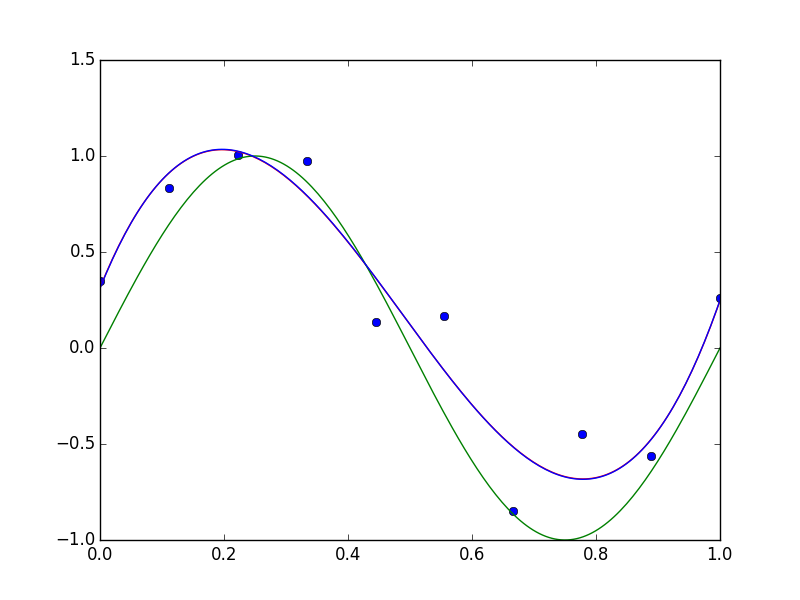
\includegraphics[scale=0.4]{figure2_1.png}
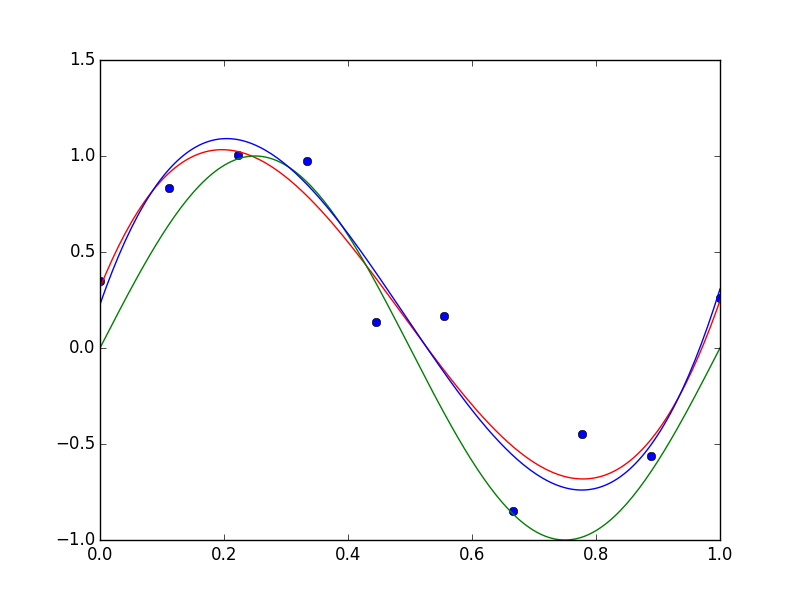
\includegraphics[scale=0.4]{figure2_2.png}
\caption{The maximum-likelihood polynomials ($M=3$) produced by gradient descent. The sin function used to generate the data is in green, the polynomial produced by the closed-form formula in red, and the polynomial produced by gradient descent in blue. Note that in the left figure, the red curve is almost invisible, as it is mostly covered by the blue curve. The figure on the left corresponds to a convergence criterion of $10^{-8}$, while the one on the right corresponds to a convergence criterion of $10^{-5}$. The \texttt{fmin\_bfgs} function produced a figure similar to the one on the left.}
\end{figure}

Because the data set that we used was generated using an underlying sin function, we investigated the behavior of the algorithm when trigonometric functions were used to generate $\Phi$. We initially expected that the algorithm would generate a fit that was closer to the original sin function, but it actually did not. The result of this can be seen in Figure \ref{p2figure2}. Attempting to fit data in this way without knowing how it was generated also carries some disadvantages. Any function that we generate with trigonometric basis functions must necessarily be periodic with period 1, so the fit may not generalize well to values of $x$ outside the interval supplied. Furthermore, trigonometric functions will have a difficult time characterizing simple relationships, such as linear correlations.

\begin{figure}
\label{p2figure2}
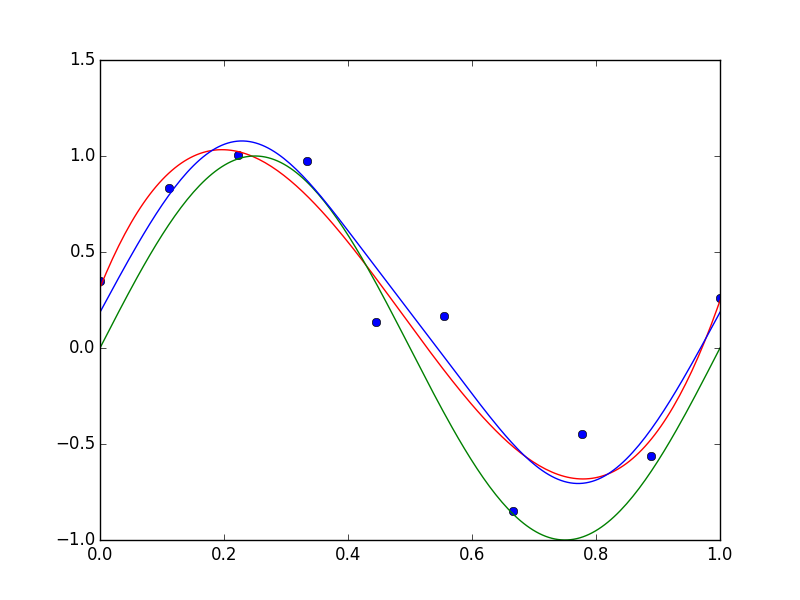
\includegraphics[scale=0.4]{figure2_3.png}
\caption{The maximum-likelihood function produced using trigonometric basis functions ($M=3$). This function (blue) does not actually appear to be more faithful to the original sin function (green) than the maximum-likelihood degree-3 polynomial (red).}
\end{figure}

\section{Least Absolute Deviation}
Alternatively to minimizing the SSE in a regression problem, we can instead try to minimize the sum of the absolute errors, which is a method called Least Absolute Deviation (i.e. LAD). In this section we investigate the behavior of this method of optimization.

We repeated our experiment from section 3 in this section, fitting weight vectors for values of $M$ between 0 and 9 (inclusive), and values of $\lambda$ of the form $2^{k/2}$ for integers $-3 \le k \le 11$. We found the cross-validation error for each weight vector, and discovered that $(M, \lambda) = (2, 2^{-3})$ resulted in the lowest cross-validation error, while $(M, \lambda) = (6, 2^{-1})$ resulted in the highest. However, the best and worst CV errors differed by only one order of magnitude, which surprised us. We believe this is due to an affinity towards median behavior of this method, as the value with the least absolute error with respect to a set of values is the median of that set. The best and worst fits are depicted in Figure \ref{p4figure}.

\begin{figure}
\label{p4figure}
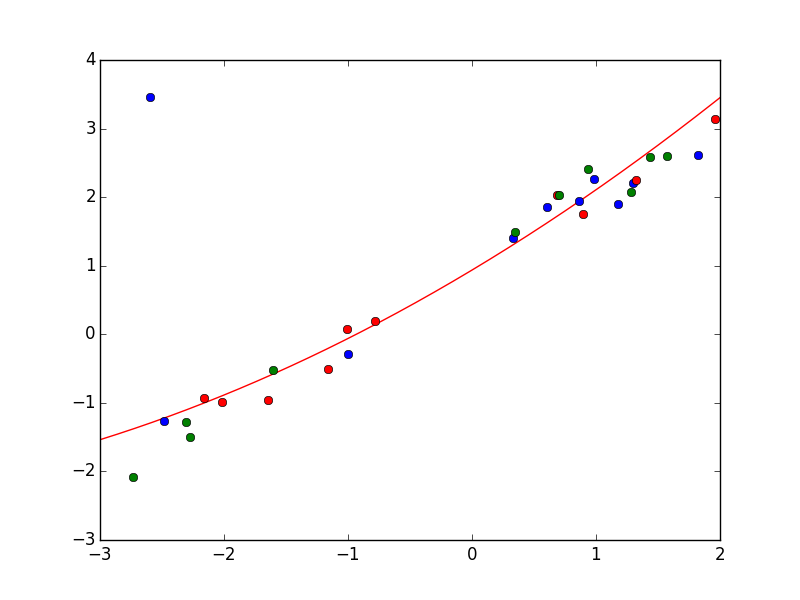
\includegraphics[scale=0.4]{figure4_3.png}
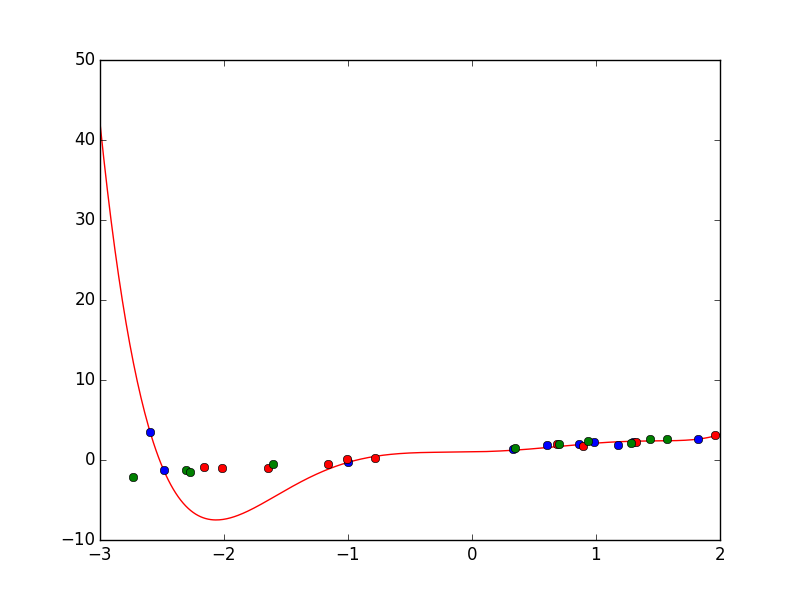
\includegraphics[scale=0.4]{figure4_4.png}
\caption{The fits with the lowest (left) and highest (right) cross-validation errors. The left fit used the values $M=2, \lambda = 2^{-3}$, while the right fit used the values $M=6, \lambda = 2^{-1}$. The fitted polynomial is shown in red, with the training set, cross-validation set, and test set shown in blue, red, and green, respectively.}
\end{figure}

Upon looking at all of the generated data, it appeared that the value of $\lambda$ had little consequence on the cross-validation error, and that there was at best a slight positive relationship between the value of $M$ and the cross-validation error. It thus seems that using ridge regression has little consequence when using LAD. Ridge regression seems more suitable in situations where overfitting may be a problem, and because LAD demonstrates affinity for median-like behavior, it is unlikely to overfit. We believe that LAD is a suitable method to use when other methods, such as ridge regression, are insufficient for solving the overfitting problem, or when finding optimal values of $M$ and $\lambda$ is impractical (many values to try, large datasets that take a long time to fit, etc.).
\end{document}
